\documentclass[12pt]{article}
\usepackage[margin=1in]{geometry} 
\usepackage{amsmath,amsthm,amssymb,amsfonts}
\usepackage{romannum}
\usepackage{dsfont}
\usepackage{graphicx}
 
\newcommand{\N}{\mathbb{N}}
\newcommand{\Z}{\mathbb{Z}}
 
\newenvironment{problem}[2][Problem]{\begin{trivlist}
\item[\hskip \labelsep {\bfseries #1}\hskip \labelsep {\bfseries #2.}]}{\end{trivlist}}
%If you want to title your bold things something different just make another thing exactly like this but replace "problem" with the name of the thing you want, like theorem or lemma or whatever

\renewcommand\thesubsubsection{\arabic{subsubsection}}
\renewcommand{\vec}[1]{\mathbf{#1}}
 
\begin{document}
 
%\renewcommand{\qedsymbol}{\filledbox}
%Good resources for looking up how to do stuff:
%Binary operators: http://www.access2science.com/latex/Binary.html
%General help: http://en.wikibooks.org/wiki/LaTeX/Mathematics
%Or just google stuff
 
\title{SLAM \Romannum{2}}
\date{\vspace{-20mm}}
\maketitle

\section*{EKF SLAM via the MonoSLAM example} 

\subsection*{EKF SLAM via the MonoSLAM example}

This exercise is designed to exercise your understanding of the EKF SLAM equations and their meaning. In particular, here we are looking at EKF SLAM via the MonoSLAM system [Davison et al.,PAMI 2007] we discussed in this week's lecture segments. \\

\begin{figure}[h]
	\centering
	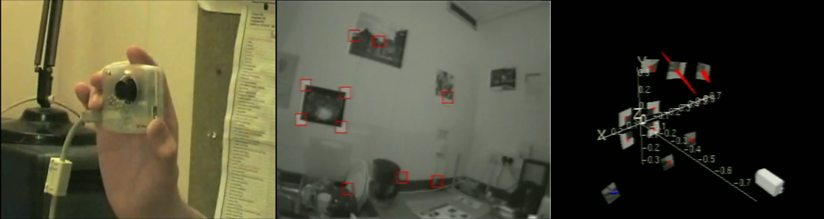
\includegraphics[width=0.8\linewidth]{monoslam_snapshot}
	\caption{MonoSLAM IN ACTION: the external view, the camera view and the SLAM map}
\end{figure}

\noindent Following the notation of MonoSLAM, vector $\vec{x}$ stacks the state of the camera and the landmarks $\vec{y}_i$ and the associated covariance matrix $\mathbf{P}$ encodes the variance in and correlation across the individual elements of $\vec{x}$. Below, is a set of partially completed equations to perform EKF SLAM. Read on carefully and select the option that substitutes the \# symbol, such that these equations are completed correctly. \\

\noindent Note: the hat ( $\hat{}$ ) symbol denotes a predicted value (e.g. $\hat{\vec{x}}$) and the subcripts on $\vec{x}$ and $\mathbf{P}$ correspond to different time-stamps (e.g. $\vec{x}_t$ is the state at time $t$). \\

\noindent What does the \# correspond to in each equation?

\subsubsection*{Prediction Step}

Let $f$ denote the prediction function and $\vec{u}_t$ denote the odometric/control input between time-stamps $t−1$ and $t$ (assuming that it is available).

\begin{equation}
	\vec{\hat{x}}_t = f(\vec{x}_{t-1}, \vec{u}_t)
\end{equation}

\noindent Let $\mathbf{F_x}$ and $\mathbf{F_u}$ denote the Jacobians of function $f$ (above) with respect to $\vec{x}$ and $\vec{u}$, respectively and $\mathbf{Q_t}$ the covariance matrix corresponding to $\vec{u}_t$.

\begin{equation}
	\mathbf{\hat{P}_t} = \mathbf{F_x} \mathbf{P_{t-1}} \mathbf{F_x}^T + \mathbf{F_u} \mathbf{Q_t} \mathbf{F_u}^T
\end{equation}

\subsubsection*{Measurement Step}

Let $\vec{h_i}$ denote the measurement projection function for feature $\vec{y_i}$.

\begin{equation}
	\vec{\hat{z}_i} = h_i(\vec{\hat{x}}_t, \vec{y_i})
\end{equation}

\noindent If $\mathbf{H}$ is the Jacobian of h with respect to $\vec{x}$ and $\mathbf{R}$ the constant noise covariance of measurements, then the innovation covariance matrix $\mathbf{S}$ is defined as,

\begin{equation}
	\mathbf{S} = \mathbf{H} \mathbf{\hat{P}_t} \mathbf{H}^T + \mathbf{R}
\end{equation}


\subsubsection*{Update Step}

If the Kalman gain at time $t$ corresponds to:

\begin{equation*}
	\mathbf{K_t} = \mathbf{\hat{P}_t} \mathbf{H} \mathbf{S}^{-1} 
\end{equation*}

\noindent then

\begin{equation}
	\vec{x_t} = \vec{\hat{x}_t} + \mathbf{K_t} (\vec{z_{0:n}} - \vec{\hat{z}_{0:n}})
\end{equation}

\begin{equation}
	\mathbf{P_t} = \mathbf{\hat{P}_t} - \mathbf{K_t} \mathbf{S} \mathbf{K_t}^T
\end{equation}


\end{document}